\documentclass[12pt]{article}
\usepackage[utf8]{inputenc}
\usepackage[russian]{babel}
\usepackage{amsmath, amssymb, amsthm}
\usepackage{graphicx}
\usepackage{float}
\usepackage{caption}
\usepackage{subcaption}
\usepackage{siunitx}
\usepackage{booktabs}
\usepackage{multirow}
\usepackage[a4paper, margin=2cm]{geometry}
\usepackage{physics}
\author{Струков Олег, Б04-404}
\title{Различные типы электронной эмиссии}

\date{}

\begin{document}

\maketitle

\section*{Определение}
Электронная эмиссия -- процесс выхода электронов из твёрдого тела в вакуум или другую среду. Основным параметром, определяющим возможность эмиссии, является работа выхода $\varphi$ -- минимальная энергия, необходимая для удаления электрона из тела. Явление электронной эмиссии лежит в основе работы множества современных устройств: от традиционных вакуумных ламп до электронных микроскопов и ускорителей частиц. 



\section*{Основные типы электронной эмиссии}
Существует несколько основных механизмов электронной эмиссии, различающихся по источнику энергии, обеспечивающему преодоление потенциального барьера:

\begin{enumerate}
    \item \textbf{Термоэлектронная эмиссия (ТЭЭ)}: Нагрев катода приводит к тому, что часть электронов приобретает энергию, достаточную для преодоления работы выхода. Это наиболее широко используемый механизм в вакуумной электронике.
    
    \item \textbf{Автоэлектронная (туннельная, полевая) эмиссия}: Сильное внешнее электрическое поле ($\sim 10^9 \text{ В}\cdot\text{м}^{-1}$) понижает потенциальный барьер, что позволяет электронам туннелировать через него при комнатной температуре.
    
    \item \textbf{Фотоэлектронная эмиссия}: Поглощение фотона с энергией $h\nu > \varphi$ приводит к выбиванию электронов из материала.
    
    \item \textbf{Вторичная электронная эмиссия}: Бомбардировка поверхности первичными электронами или ионами приводит к выбиванию вторичных электронов.
\end{enumerate}

\begin{table}[H]
    \centering
    % \caption{Сравнительные характеристики различных типов электронной эмиссии}
    \begin{tabular}{lccc}
        \toprule
        Тип эмиссии & Источник энергии & Плотность тока & Температура  \\
        \midrule
        Термоэлектронная & Тепловая & от 0,1 до 10 $\text{А}\cdot\text{см}^{-2}$ & $> 1000$ К  \\
        Автоэлектронная & Электрич. поле & от 10$^4$ до 10$^9$ $\text{А}\cdot\text{см}^{-2}$ & $\sim 300$ К  \\
        Фотоэлектронная & Свет & от 0,01 до 1 $\text{мА}\cdot\text{см}^{-2}$ & Любая  \\
        Вторичная & Кинетическая & $\propto$ первич. току & Любая \\
        \bottomrule
    \end{tabular}
    \label{tab:emission_types}
\end{table}

\newpage
\section*{Термоэлектронная эмиссия}
Термоэлектронная эмиссия описывается распределением Ферми--Дирака. При нагреве материала катода часть электронов приобретает энергию, превышающую уровень вакуума, и может покинуть материал. Зависимость плотности тока термоэмиссии от температуры и работы выхода описывается формулой Ричардсона--Дэшмана:

\begin{equation}
    j = A T^2 e^{-\varphi / kT}, \quad A = \frac{4\pi m e k^2}{h^3} \approx 120 \text{А}\cdot\text{см}^{-2}\cdot\text{К}^{-2}
    \label{eq:richardson}
\end{equation}

где $A$ -- теоретическая постоянная Ричардсона, $m$ -- масса электрона, $e$ -- заряд электрона, $k$ -- постоянная Больцмана, $h$ -- постоянная Планка.

Формула Ричардсона-Дэшмана получается путём статистического подсчёта числа электронов, которые имеют достаточно энергии для преодоления потенциального барьера и движутся в правильном направлении -- в сторону поверхности.

Множитель $T^2$ в формуле возникает по двум причинам: 1) плотность состояний электронов у верхнего края потенциальной ямы пропорциональна $T$, 2) средняя скорость электронов также пропорциональна $T$.%, что даёт общую зависимость $T^2$.

\subsection*{Поправки к формуле Ричардсона--Дэшмана}
\textbf{Эффект Шоттки} -- снижение работы выхода при наличии внешнего ускоряющего поля $E$:

\begin{equation}
    \Delta\varphi = \sqrt{e^3 E} \quad\text{ [СГСЭ]}, \quad \Delta\varphi = \sqrt{\frac{e^3 E}{4\pi\varepsilon_0}} \quad \text{ [СИ]}
    \label{eq:schottky_cgs}
\end{equation}
где $e$ -- заряд электрона, $E$ -- напряжённость электрического поля. 

Учёт эффекта Шоттки приводит к следующей формуле:

\begin{equation}
    j = A T^2 e^{-(\varphi - \Delta\varphi)/kT}
    \label{eq:schottky_richardson}
\end{equation}

\begin{figure}[H]
    \centering
    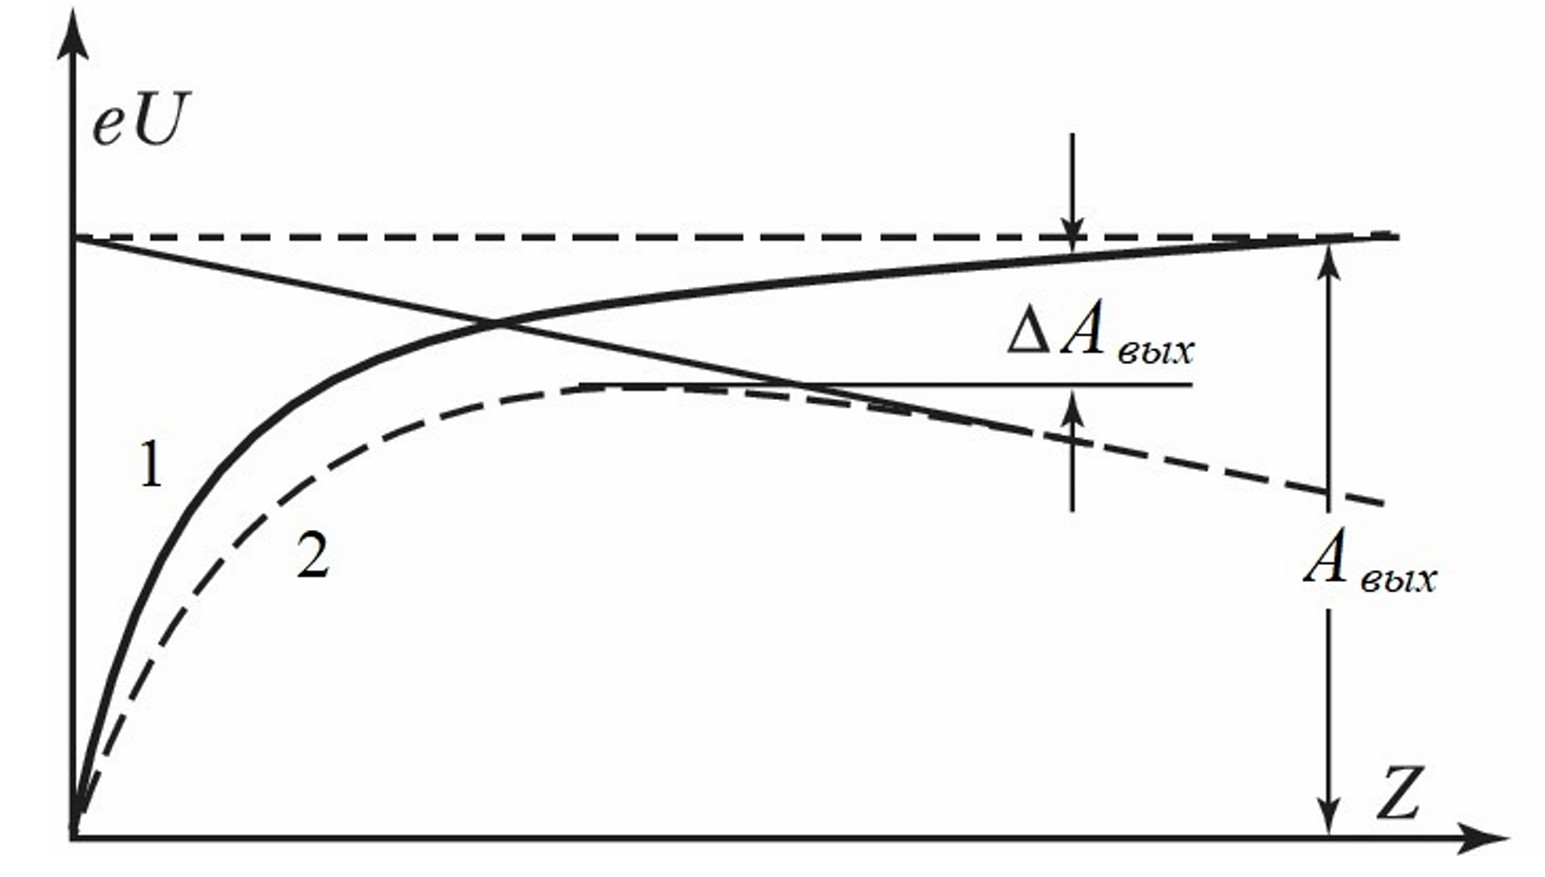
\includegraphics[width=0.6\textwidth]{Работа выхода.jpg}
    \caption{Распределение потенциала у поверхности  
металла при отсутствии (кривая 1) и наличии (кривая 2)  
внешнего ускоряющего электрического поля; А$_{\text{вых}}$ -- полная  
работа выхода; Z -- расстояние от эмитирующей поверхности}
    \label{fig:barrier}
\end{figure}

\textbf{Эффективная постоянная $A^*$} отличается от теоретического значения из-за отражения электронов от потенциального барьера и неоднородности поверхности катода.

\newpage

\textbf{Температурная зависимость работы выхода}

Работа выхода $\varphi$ не является строго постоянной -- она зависит от температуры из-за теплового расширения кристаллической решётки, изменения уровня Ферми и поверхностных эффектов. В первом приближении:

\begin{equation}
    \varphi(T) \approx \varphi_0 + \beta T,
    \label{eq:phi_temp}
\end{equation}

где $\varphi_0$ -- экстраполированное значение при $T \to 0$, коэффициент $\beta \sim 10^{-4} - 10^{-5}\ \text{эВ/К}$. С учётом этой поправки формула принимает вид:

\begin{equation}
    j = A T^2 e^{-(\varphi_0 + \beta T)/kT} %= A T^2 e^{-\varphi_0/kT} e^{-\beta/k}.
    \label{eq:richardson_temp_corrected}
\end{equation}

% На графике Ричардсона $\ln(j/T^2)$ от $1/T$ эта поправка проявляется как нелинейность и влияет на измеряемое значение $A^*$.

\vspace{0.5cm}

\textbf{Квантово-статистическая поправка (функция Нордхейма)}

В исходном выводе используется приближение Больцмана для хвоста распределения Ферми-Дирака. Более строгий учёт даёт поправочный множитель -- \emph{функцию Нордхейма} $F_N(w)$, где $w = (\varphi - E_F)/kT$, а $E_F$ -- уровень Ферми электронного газа в металле:

\begin{equation}
    F_N(w) \approx 1 - \frac{\pi^2}{6} \left(\frac{kT}{\varphi - E_F}\right)^2 + \ldots \quad \text{при } w \gg 1.
    \label{eq:nordheim_func}
\end{equation}

С этой поправкой формула записывается как:

\begin{equation}
    j = A T^2 \, F_N\!\left(\frac{\varphi - E_F}{kT}\right) e^{-\varphi/kT}.
    \label{eq:richardson_nordheim}
\end{equation}

При высоких температурах или малой $\varphi$ поправка становится существенной и объясняет часть расхождения между теоретическим $A$ и экспериментальным $A^*$.

\vspace{0.5cm}

\textbf{Общий вид с основными поправками}

Учёт эффекта Шоттки, температурной зависимости $\varphi(T)$ и функции Нордхейма приводит к обобщённой формуле:

\begin{equation}
    j = A^* T^2 \, F_N\!\left(\frac{\varphi_0 + \beta T - E_F}{kT}\right) 
        \, e^{-(\varphi_0 + \beta T - \Delta\varphi)/kT}.
    \label{eq:richardson_general}
\end{equation}


\subsection*{Автоэлектронная эмиссия}
Формула Фаулера-Нордхейма для плотности тока через потенциальный барьер в сильном электрическом поле $E$:
\begin{equation}
    j = \frac{e^3 E^2}{8\pi h \varphi} \exp\left[-\frac{4\sqrt{2m}\,\varphi^{3/2}}{3\hbar e E}\right],
    \label{eq:fn_emission}
\end{equation}
где $\varphi$ -- работа выхода, $e$ -- заряд электрона, $m$ -- масса электрона, $\hbar = h/2\pi$ -- приведённая постоянная Планка.

\subsection*{Фотоэлектронная эмиссия}
Закон Эйнштейна для внешнего фотоэффекта, определяющий максимальную кинетическую энергию фотоэлектронов:
\begin{equation}
    E_k^{\text{max}} = h\nu - \varphi,
    \label{eq:photo_emission}
\end{equation}
где $h\nu$ -- энергия падающего фотона. Плотность фототока пропорциональна интенсивности света и зависит от $\nu$ и $\varphi$.

\subsection*{Вторичная электронная эмиссия}
Коэффициент вторичной эмиссии (основная характеристика):
\begin{equation}
    \delta = \frac{I_s}{I_p} = f(E_p, \theta, \text{материал}),
    \label{eq:secondary_emission}
\end{equation}
где $I_s$ -- ток вторичных электронов, $I_p$ -- ток первичных электронов, $E_p$ -- их энергия, $\theta$ -- угол падения. 
Типичная зависимость $\sigma(E_p)$ имеет максимум при $E_p \sim 100\!-\!1000$ эВ.




\section*{Сравнение эффективности различных типов электронной эмиссии при фиксированном ускоряющем напряжении}

\subsection*{Исходные параметры}
\begin{itemize}
    \item Ускоряющее напряжение: $U_a = 10$ кВ
    \item Работа выхода (для термо- и автоэмиссии): $\varphi = 4,5$ эВ
    \item \textbf{Термоэмиссия:} материал -- вольфрам, постоянная Ричардсона $A = 120$ А·см$^{-2}$·К$^{-2}$, коэффициент излучения $\varepsilon = 0,3$
    \item \textbf{Автоэмиссия:} рассматривается плоская геометрия катода, задана реалистичная плотность тока $j_F = 10^4$ А/см$^2$, характерная для стабильной работы матриц наноэмиттеров
    \item \textbf{Фотоэмиссия:} длина волны излучения $\lambda = 250$ нм ($h\nu = 4,96$ эВ), квантовая выходность $Y = 0,1$ эл/фотон
\end{itemize}

\subsection*{Метод сравнения}
Для каждого механизма эмиссии рассчитывается ток $I$, который может быть получен при реализации физически достижимых параметров. Мощность $P$ определяется как мощность, непосредственно подводимая к катоду для поддержания эмиссии: для термоэмиссии -- мощность нагрева, для автоэмиссии -- электрическая мощность источника высокого напряжения ($P = I \cdot U_a$), для фотоэмиссии -- мощность оптического излучения. Эффективность рассчитывается как $\eta = I/P$.

\subsection*{Расчёты}

\noindent\textbf{1. Термоэмиссия (вольфрамовый катод)}

Оптимальная температура для вольфрама: $T = 2800$ К. Плотность термоэмиссионного тока:
\[
j_T = A T^2 e^{-\varphi/kT} = 120 \cdot (2800)^2 \cdot e^{-4,5/(8.617\cdot10^{-5} \cdot 2800)} \approx 7,0\ \text{А/см}^2.
\]

Зададим площадь катода $S_T = 1$ см$^2$, тогда полный ток:
\[
I_T = j_T \cdot S_T \approx 7,0\ \text{А}.
\]

Мощность, необходимая для нагрева катода до 2800 К (с учётом только излучательных потерь):
\[
P_T = \varepsilon \sigma_S T^4 S_T = 0,3 \cdot 5,67\cdot10^{-8} \cdot (2800)^4 \cdot 10^{-4} \approx 104,6\ \text{Вт}.
\]

Эффективность:
\[
\eta_T = \frac{I_T}{P_T} \approx \frac{7,0}{104,6} \approx 0,067\ \text{А/Вт}.
\]

\noindent\textbf{2. Автоэмиссия (плоский катод)}

Зададим плотность тока $j = 10^4$ А/см$^2 = 10^8$ А/м$^2$. Из формулы Фаулера--Нордхейма для плоского катода:
\[
j = \frac{A_{\text{FN}} E^2}{\varphi} \exp\left(-\frac{B_{\text{FN}} \varphi^{3/2}}{E}\right),
\]
где $A_{\text{FN}} = 1,54\cdot10^{-6}$ А·эВ·В$^{-2}$, $B_{\text{FN}} = 6,83\cdot10^9$ В·м$^{-1}$·эВ$^{-3/2}$. Численное решение даёт необходимую напряжённость поля $E \approx 5,75\cdot10^9$ В/м.

При ускоряющем напряжении $U_a = 10$ кВ требуемое расстояние между катодом и анодом:
\[
d = \frac{U_a}{E} = \frac{10^4}{5,75\cdot10^9} \approx 1,74\ \text{мкм}.
\]

Выберем мощность источника $P = 100$ Вт. Тогда ток:
\[
I = \frac{P}{U_a} = \frac{100}{10^4} = 0,01\ \text{А}.
\]

Необходимая площадь эмиттера:
\[
S = \frac{I}{j} = \frac{0,01}{10^4} = 10^{-6}\ \text{см}^2 = 10^{-10}\ \text{м}^2.
\]

Эффективность:
\[
\eta = \frac{I}{P} = 10^{-4}\ \text{А/Вт}.
\]

\noindent\textbf{3. Фотоэмиссия}

Мощность оптического излучения, падающего на фотокатод: $P = 100$ Вт. Полный фотоэмиссионный ток:
\[
I = \frac{e P Y}{h\nu} = \frac{1,6\cdot10^{-19} \cdot 100 \cdot 0,1}{4,96 \cdot 1,6\cdot10^{-19}} \approx 2,0\ \text{А}.
\]

Для исключения теплового разрушения в непрерывном режиме ограничим плотность мощности излучения величиной $p = 1$ Вт/см$^2$. Тогда необходимая площадь фотокатода:
\[
S = \frac{P}{p} = \frac{100}{1} = 100\ \text{см}^2.
\]

Плотность фототока:
\[
j = \frac{I}{S} = 0,02\ \text{А/см}^2 \quad \Rightarrow  \quad \eta = \frac{I}{P} = 0,02\ \text{А/Вт}.
\]

\subsection*{Сравнительная таблица}
\begin{table}[H]
\centering
\begin{tabular}{|l|c|c|c|c|}
\hline
\textbf{Тип эмиссии} & \textbf{Ток, А} & \textbf{Плотность тока} & \textbf{Площадь, см$^2$} & \textbf{Эффективность, А/Вт} \\
\hline
Термоэмиссия & 7,0 & $7,0$ А/см$^2$ & 1,0 & 0,067 \\
\hline
Автоэмиссия & 0,01 & $10^4$ А/см$^2$ & 10$^{-6}$ & 1,0$\cdot10^{-4}$ \\
\hline
Фотоэмиссия & 2,0 & $0,02$ А/см$^2$ & 100 & 0,020 \\
\hline
\end{tabular}
\label{tab:comparison_Ua}
\end{table}

% \subsection*{Обсуждение результатов}
% \begin{itemize}
%     \item \textbf{Термоэмиссия} демонстрирует наибольшие значения тока и эффективности преобразования мощности накачки в ток эмиссии. Это связано с относительно низкой мощностью, требуемой для нагрева катода, и умеренной, но значительной плотностью эмиссионного тока. Основные ограничения -- высокотемпературная эксплуатация и сравнительно невысокая плотность тока.

%     \item \textbf{Автоэмиссия} обладает исключительно высокой плотностью тока, но достигается это ценой крайне низкой общей эффективности. Низкая эффективность $\eta_F = 1/U_a$ является фундаментальным ограничением, связанным с необходимостью приложения высокого ускоряющего напряжения для создания полей туннелирования. Получаемые токи малы, а требуемые площади эмиссии ничтожны, что делает данный механизм малопригодным для генерации больших токов, но перспективным для применения в случаях, когда необходима высокая плотность тока на ультрамалой площади.

%     \item \textbf{Фотоэмиссия} занимает промежуточное положение. Она позволяет получать значительные токи, но требует большой площади фотокатода из-за тепловых ограничений, что приводит к низкой плотности тока. Эффективность преобразования световой мощности в ток существенно превышает эффективность автоэмиссии, но уступает термоэмиссии.

% \end{itemize}

\textbf{Вывод:} При фиксированном ускоряющем напряжении наиболее эффективным механизмом для получения больших токов является термоэмиссия. Автоэмиссия, несмотря на наибольшую плотность тока, характеризуется низкой эффективностью. Фотоэмиссия представляет собой средний вариант, требующий больших площадей катода.

% Дополнительное примечание о КПД
% \paragraph*{Примечание о КПД преобразования}
% Для термо- и фотоэмиссии можно дополнительно определить КПД преобразования мощности накачки в энергию ускоренного пучка, если задать ускоряющее напряжение $U_a$, общее для всех механизмов. Однако для автоэмиссии напряжение $V$ одновременно определяет и эмиссию, и ускорение, что делает прямое сравнение КПД по формуле $\eta = I U_a / P$ физически некорректным. Поэтому в качестве универсальной сравнительной метрики использован ток на ватт ($I/P$).

% \noindent\textbf{Вывод:} Наибольший ток при заданной мощности обеспечивает термоэмиссия, автоэмиссия даёт максимальную плотность тока, фотоэмиссия демонстрирует лучший КПД при использовании эффективных фотокатодов.



\section*{Заключение}

\subsection*{Достоинства и недостатки различных типов электронной эмиссии}

\begin{itemize}
    \item \textbf{Термоэмиссия} обеспечивает устойчивые токи высокой плотности, но требует энергозатратного нагрева и имеет ограниченный срок службы из-за испарения материала катода.    
    \item \textbf{Автоэмиссия} даёт наибольшие плотности тока при комнатной температуре, но требует очень высоких напряжённостей поля и чувствительна к состоянию поверхности.
    \item \textbf{Фотоэмиссия} позволяет управлять током модуляцией светового потока, но требует источников излучения с энергией фотонов, превышающей работу выхода.
    \item \textbf{Вторичная эмиссия} эффективна для усиления слабых сигналов, но коэффициент вторичной эмиссии обычно невелик ($\delta < 10$ для большинства материалов).
\end{itemize}

\subsection*{Практическое применение}
\begin{itemize}
    \item \textbf{Термоэмиссия} широко используется в вакуумных лампах, СВЧ-генераторах (клистроны, магнетроны), электронных пушках микроскопов и ионных двигателях.
    \item \textbf{Автоэмиссия} применяется в полевых эмиттерах для растровых электронных микроскопов и наноэлектронных устройствах.
    \item \textbf{Фотоэмиссия} лежит в основе фотоэлектронных умножителей и спектроскопии.
    \item \textbf{Вторичная эмиссия} используется для усиления электронных сигналов и для отображения информации на ЭЛТ-мониторах.
\end{itemize}
Различные типы электронной эмиссии применяются в зависимости от конкретных условий и требований к приборам. Термоэлектронная эмиссия является основным механизмом для приборов, требующих высоких и стабильных токов, несмотря на энергозатратность нагрева.



\subsection*{Используемая литература}
\begin{enumerate}
    \item Батурин А.С., Кириченко Л.А. и др. / Эмиссионная электроника в примерах и задачах: Учебное пособие.
    \item Сивухин Д.В. / Общий курс физики.
    \item Зенин А.А. и др. / Вакуумная и плазменная электроника: учеб. пособие для аспирантов направления 11.06.01.
    \item В. М. Агафонов, Е. П. Шешин. / Термоэлектронный диод: лабораторная работа по курсу Вакуумная электроника.
\end{enumerate}
\end{document}